%\VignetteEngine{knitr::knitr}

\documentclass[a4paper,10pt]{article}\usepackage[]{graphicx}\usepackage[]{color}
%% maxwidth is the original width if it is less than linewidth
%% otherwise use linewidth (to make sure the graphics do not exceed the margin)
\makeatletter
\def\maxwidth{ %
  \ifdim\Gin@nat@width>\linewidth
    \linewidth
  \else
    \Gin@nat@width
  \fi
}
\makeatother

\definecolor{fgcolor}{rgb}{0.345, 0.345, 0.345}
\newcommand{\hlnum}[1]{\textcolor[rgb]{0.686,0.059,0.569}{#1}}%
\newcommand{\hlstr}[1]{\textcolor[rgb]{0.192,0.494,0.8}{#1}}%
\newcommand{\hlcom}[1]{\textcolor[rgb]{0.678,0.584,0.686}{\textit{#1}}}%
\newcommand{\hlopt}[1]{\textcolor[rgb]{0,0,0}{#1}}%
\newcommand{\hlstd}[1]{\textcolor[rgb]{0.345,0.345,0.345}{#1}}%
\newcommand{\hlkwa}[1]{\textcolor[rgb]{0.161,0.373,0.58}{\textbf{#1}}}%
\newcommand{\hlkwb}[1]{\textcolor[rgb]{0.69,0.353,0.396}{#1}}%
\newcommand{\hlkwc}[1]{\textcolor[rgb]{0.333,0.667,0.333}{#1}}%
\newcommand{\hlkwd}[1]{\textcolor[rgb]{0.737,0.353,0.396}{\textbf{#1}}}%

\usepackage{framed}
\makeatletter
\newenvironment{kframe}{%
 \def\at@end@of@kframe{}%
 \ifinner\ifhmode%
  \def\at@end@of@kframe{\end{minipage}}%
  \begin{minipage}{\columnwidth}%
 \fi\fi%
 \def\FrameCommand##1{\hskip\@totalleftmargin \hskip-\fboxsep
 \colorbox{shadecolor}{##1}\hskip-\fboxsep
     % There is no \\@totalrightmargin, so:
     \hskip-\linewidth \hskip-\@totalleftmargin \hskip\columnwidth}%
 \MakeFramed {\advance\hsize-\width
   \@totalleftmargin\z@ \linewidth\hsize
   \@setminipage}}%
 {\par\unskip\endMakeFramed%
 \at@end@of@kframe}
\makeatother

\definecolor{shadecolor}{rgb}{.97, .97, .97}
\definecolor{messagecolor}{rgb}{0, 0, 0}
\definecolor{warningcolor}{rgb}{1, 0, 1}
\definecolor{errorcolor}{rgb}{1, 0, 0}
\newenvironment{knitrout}{}{} % an empty environment to be redefined in TeX

\usepackage{alltt}
\usepackage{amsmath,mathrsfs,graphicx}
%\usepackage[top=2cm,bottom=2cm,left=2cm,right=2cm]{geometry}
\usepackage[utf8]{inputenc}
\usepackage{color}
%\usepackage{natbib}

%\usepackage{Sweave}
\RequirePackage{/afs/cs.wisc.edu/u/z/u/zuo/R/x86_64-redhat-linux-gnu-library/3.0/BiocStyle/sty/Bioconductor}


\title{atSNP: affinity tests for regulatory SNP detection}

\author{Chandler Zuo, Sunyoung Shin and S\"und\"uz Kele\c{s}\\
Department of Statistics and of Biostatistics and Medical Informatics, University of Wisconsin Madison}
  
\date{}
\IfFileExists{upquote.sty}{\usepackage{upquote}}{}
\begin{document}
\maketitle

\tableofcontents

\section{Introduction}

This document provides an introduction to the affinity test for large sets of SNP-motif interactions using the \software{atSNP} package(\textbf{a}ffinity \textbf{t}est for regulatory \textbf{SNP} detection) \cite{zuo15}. \software{atSNP} implements in-silico methods for identifying SNPs that potentially may affect binding affinity of transcription factors. Given a set of SNPs and a library of motif position weight matrices (PWMs), \software{atSNP} provides three main functions for analyzing SNP effects:

% Not sure if is is on purpose, but the cite zuo14 is not in the bib
% file.

\begin{enumerate}
\item Computing the binding affinity score for each allele and each PWM.
\item Computing the p-values for allele-specific binding affinity scores.
\item Computing the p-values for affinity score changes between the two alleles for each SNP.
\end{enumerate}

\software{atSNP} implements the importance sampling algorithm in \cite{isample} to compute the p-values. Compared to other bioinformatics tools, such as FIMO \cite{fimo} and is-rSNP \cite{is-rsnp} that provide similar functionalities, \software{atSNP} avoids computing the p-values analytically. %This reduces the execution time drastically because the probability sample space is a exponential order of the motif length. 
In one of our research projects, we have used atSNP to evaluate interactions between 26K SNPs and 2K motifs within 5 hours. We found no other existing tool can finish the analysis of such a scale.

% I didn't understood the last statement, I think it means it is
% O(exp(L)) where L is the motif length. However, based on Sunduz
% comment on the email I am not sure it this even necessary, since the
% package is aimed to users without R knowledge they may just want to
% know that atSNP is fast but not why

\section{Installation}

We are working to make the package available through bioconductor. The developing version can be installed from the Github repository:

\begin{knitrout}
\definecolor{shadecolor}{rgb}{0.969, 0.969, 0.969}\color{fgcolor}\begin{kframe}
\begin{alltt}
\hlkwd{library}\hlstd{(devtools)}
\hlkwd{install_github}\hlstd{(}\hlstr{"chandlerzuo/atSNP"}\hlstd{)}
\end{alltt}
\end{kframe}
\end{knitrout}

% The following dependent \R{} packages are required:
\software{atSNP} depends on the following \R{} packages:

\begin{itemize}
\item \CRANpkg{data.table} is used for formatting results that are easy for users to query.
\item \Biocpkg{motifStack} is relied upon to draw sequence logo plots.
\item \CRANpkg{doMC} is used for parallel computation.
\item \CRANpkg{Rcpp} interfaces the C++ codes that implements the importance sampling algorithm.
\end{itemize}
  
In addition, users need to install the annotation package \Biocannopkg{BSgenome} from \url{www.bioconductor.org/packages/3.0/data/annotation/} that corresponds to the species type and genome version. Our example SNP data set in the subsequent sections corresponds to the hg19 version of human genome. To repeat the sample codes in this vignette, the \Biocannopkg{BSgenome.Hsapiens.UCSC.hg19} package is required. If users wish to annotate the SNP location and allele information given their rs ids, they also need install the corresponding \Biocannopkg{SNPlocs} package. The sample codes in this vignettes require the package \Biocannopkg{SNPlocs.Hsapiens.dbSNP.20120608}. To install these packages from the \Bioconductor{} repository,
% This just makes the code appear in pretty format

\begin{knitrout}
\definecolor{shadecolor}{rgb}{0.969, 0.969, 0.969}\color{fgcolor}\begin{kframe}
\begin{alltt}
  \hlkwd{source}\hlstd{(}\hlstr{"http://bioconductor.org/biocLite.R"}\hlstd{)}
  \hlkwd{biocLite}\hlstd{(}\hlstr{"BSgenome.Hsapiens.UCSC.hg19"}\hlstd{)}
  \hlkwd{biocLite}\hlstd{(}\hlstr{"SNPlocs.Hsapiens.dbSNP.20120608"}\hlstd{)}
\end{alltt}
\end{kframe}
\end{knitrout}

% This is what actually runs the code



Notice that the annotation packages are usually large and this installation step may take a substantial amount of time.

% In this section, there are several references to bioconductor
% packages. I think that biocstyle would add the links but in the
% vignette's current version it would be useful to add link to this
% packages and perhaps add a code chunk explaining how to install both
% annotation and BSgenome.Hsapiens.UCSC.hg19 packages, and with an
% explicit warning that installing this two packages may take some
% time (as I recall those are heavy ones)


\section{Example}

\subsection{Load motif and SNP data}

\software{atSNP} provides a default motif library downloaded from \url{compbio.mit.edu/encode-motifs/motifs.txt}. This library contains 2065 known and discovered motifs from ENCODE TF ChIP-seq data sets. The following commands allows to load this motif library:

% It may be useful to specify that each element of encode_motif is a
% PWM. And it may be useful to show the actual motif sequence, since
% it may be hard to understand the matrix. Perhaps specifiy which
% columns is which nucleotide, for example jaspar's input is like:

% A [13 13 3 1 54 1 1 1 0 3 2 5 ]
% C [13 39 5 53 0 1 50 1 0 37 0 17 ]
% G [17 2 37 0 0 52 3 0 53 8 37 12 ]
% T [11 0 9 0 0 0 0 52 1 6 15 20 ]

% I added this chunck to avoid unnecesary echo's in documents
% that way only loads atSNP



\begin{knitrout}
\definecolor{shadecolor}{rgb}{0.969, 0.969, 0.969}\color{fgcolor}\begin{kframe}
\begin{alltt}
\hlkwd{library}\hlstd{(atSNP)}
\end{alltt}


{\ttfamily\noindent\itshape\color{messagecolor}{\#\# Loading required package: Rcpp\\\#\# Loading required package: data.table\\\#\# \\\#\# Attaching package: 'data.table'\\\#\# \\\#\# The following object is masked from 'package:GenomicRanges':\\\#\# \\\#\#\ \ \ \  last\\\#\# \\\#\# Loading required package: doMC\\\#\# Loading required package: foreach\\\#\# Loading required package: iterators\\\#\# Loading required package: motifStack\\\#\# Loading required package: grImport\\\#\# Loading required package: grid\\\#\# Loading required package: XML\\\#\# Loading required package: MotIV\\\#\# \\\#\# Attaching package: 'MotIV'\\\#\# \\\#\# The following object is masked from 'package:stats':\\\#\# \\\#\#\ \ \ \  filter\\\#\# \\\#\# Loading required package: ade4\\\#\# \\\#\# Attaching package: 'ade4'\\\#\# \\\#\# The following object is masked from 'package:BSgenome':\\\#\# \\\#\#\ \ \ \  score\\\#\# \\\#\# The following object is masked from 'package:Biostrings':\\\#\# \\\#\#\ \ \ \  score\\\#\# \\\#\# The following object is masked from 'package:GenomicRanges':\\\#\# \\\#\#\ \ \ \  score\\\#\# \\\#\# The following object is masked from 'package:IRanges':\\\#\# \\\#\#\ \ \ \  score}}\end{kframe}
\end{knitrout}

\begin{knitrout}
\definecolor{shadecolor}{rgb}{0.969, 0.969, 0.969}\color{fgcolor}\begin{kframe}
\begin{alltt}
\hlkwd{data}\hlstd{(encode_library)}
\hlkwd{length}\hlstd{(encode_motif)}
\end{alltt}
\begin{verbatim}
## [1] 2065
\end{verbatim}
\begin{alltt}
\hlstd{encode_motif[}\hlkwd{seq}\hlstd{(}\hlnum{3}\hlstd{)]}
\end{alltt}
\begin{verbatim}
## $SIX5_disc1
##              [,1]       [,2]     [,3]        [,4]
##  [1,] 8.51100e-03 4.2550e-03 0.987234 1.00000e-10
##  [2,] 9.02127e-01 1.2766e-02 0.038298 4.68090e-02
##  [3,] 4.55319e-01 7.2340e-02 0.344681 1.27660e-01
##  [4,] 2.51064e-01 8.5106e-02 0.085106 5.78724e-01
##  [5,] 1.00000e-10 4.6809e-02 0.012766 9.40425e-01
##  [6,] 1.00000e-10 1.0000e-10 1.000000 1.00000e-10
##  [7,] 3.82980e-02 2.1277e-02 0.029787 9.10638e-01
##  [8,] 9.44681e-01 4.2550e-03 0.051064 1.00000e-10
##  [9,] 1.00000e-10 1.0000e-10 1.000000 1.00000e-10
## [10,] 1.00000e-10 1.0000e-10 0.012766 9.87234e-01
## 
## $MYC_disc1
##              [,1]        [,2]        [,3]        [,4]
##  [1,] 1.73516e-01 1.05023e-01 7.21461e-01 1.00000e-10
##  [2,] 1.00000e-10 1.00000e-10 1.00000e-10 1.00000e+00
##  [3,] 1.00000e-10 1.00000e+00 1.00000e-10 1.00000e-10
##  [4,] 1.00000e+00 1.00000e-10 1.00000e-10 1.00000e-10
##  [5,] 1.00000e-10 9.58904e-01 1.00000e-10 4.10960e-02
##  [6,] 5.93610e-02 1.00000e-10 9.40639e-01 1.00000e-10
##  [7,] 1.00000e-10 1.00000e-10 1.00000e-10 1.00000e+00
##  [8,] 1.00000e-10 1.00000e-10 1.00000e+00 1.00000e-10
##  [9,] 1.00000e+00 1.00000e-10 1.00000e-10 1.00000e-10
## [10,] 1.00000e-10 7.26028e-01 1.14155e-01 1.59817e-01
## 
## $SRF_disc1
##              [,1]  [,2]  [,3]        [,4]
##  [1,] 1.00000e-10 1e+00 1e-10 1.00000e-10
##  [2,] 1.00000e-10 1e+00 1e-10 1.00000e-10
##  [3,] 4.95495e-01 1e-10 1e-10 5.04505e-01
##  [4,] 2.61261e-01 1e-10 1e-10 7.38739e-01
##  [5,] 1.00000e+00 1e-10 1e-10 1.00000e-10
##  [6,] 1.00000e-10 1e-10 1e-10 1.00000e+00
##  [7,] 7.29730e-01 1e-10 1e-10 2.70270e-01
##  [8,] 5.04505e-01 1e-10 1e-10 4.95495e-01
##  [9,] 1.00000e-10 1e-10 1e+00 1.00000e-10
## [10,] 1.00000e-10 1e-10 1e+00 1.00000e-10
\end{verbatim}
\end{kframe}
\end{knitrout}

Here, the motif library is represented by \Robject{encode\_motif},
which is a list of position weight matrices. The codes below shows the
content of one matrix as well as its IUPAC letters:

\begin{knitrout}
\definecolor{shadecolor}{rgb}{0.969, 0.969, 0.969}\color{fgcolor}\begin{kframe}
\begin{alltt}
\hlstd{encode_motif[[}\hlnum{1}\hlstd{]]}
\end{alltt}
\begin{verbatim}
##              [,1]       [,2]     [,3]        [,4]
##  [1,] 8.51100e-03 4.2550e-03 0.987234 1.00000e-10
##  [2,] 9.02127e-01 1.2766e-02 0.038298 4.68090e-02
##  [3,] 4.55319e-01 7.2340e-02 0.344681 1.27660e-01
##  [4,] 2.51064e-01 8.5106e-02 0.085106 5.78724e-01
##  [5,] 1.00000e-10 4.6809e-02 0.012766 9.40425e-01
##  [6,] 1.00000e-10 1.0000e-10 1.000000 1.00000e-10
##  [7,] 3.82980e-02 2.1277e-02 0.029787 9.10638e-01
##  [8,] 9.44681e-01 4.2550e-03 0.051064 1.00000e-10
##  [9,] 1.00000e-10 1.0000e-10 1.000000 1.00000e-10
## [10,] 1.00000e-10 1.0000e-10 0.012766 9.87234e-01
\end{verbatim}
\begin{alltt}
\hlkwd{GetIUPACSequence}\hlstd{(encode_motif[[}\hlnum{1}\hlstd{]])}
\end{alltt}
\begin{verbatim}
## [1] "GARWTGTAGT"
\end{verbatim}
\end{kframe}
\end{knitrout}

The data object \Robject{encode\_library} also contains a character vector \Robject{encode\_motifinfo} that contains detailed information for each motif.

\begin{knitrout}
\definecolor{shadecolor}{rgb}{0.969, 0.969, 0.969}\color{fgcolor}\begin{kframe}
\begin{alltt}
\hlkwd{length}\hlstd{(encode_motifinfo)}
\end{alltt}
\begin{verbatim}
## [1] 2065
\end{verbatim}
\begin{alltt}
\hlkwd{head}\hlstd{(encode_motifinfo)}
\end{alltt}
\begin{verbatim}
##                                                 SIX5_disc1 
##   "SIX5_GM12878_encode-Myers_seq_hsa_r1:MEME#1#Intergenic" 
##                                                  MYC_disc1 
##   "USF2_K562_encode-Snyder_seq_hsa_r1:MDscan#1#Intergenic" 
##                                                  SRF_disc1 
##  "SRF_H1-hESC_encode-Myers_seq_hsa_r1:MDscan#2#Intergenic" 
##                                                  AP1_disc1 
##     "JUND_K562_encode-Snyder_seq_hsa_r1:MEME#1#Intergenic" 
##                                                 SIX5_disc2 
## "SIX5_H1-hESC_encode-Myers_seq_hsa_r1:MDscan#1#Intergenic" 
##                                                  NFY_disc1 
##     "NFYA_K562_encode-Snyder_seq_hsa_r1:MEME#2#Intergenic"
\end{verbatim}
\end{kframe}
\end{knitrout}

Here, the entry names of this vector are the same as the names of the motif library. \Robject{encode\_motifinfo} allows easy looking up the motif information for a specific PWM. For example, to look up the motif information for the first PWM in \Robject{encode\_motifinfo}:

\begin{knitrout}
\definecolor{shadecolor}{rgb}{0.969, 0.969, 0.969}\color{fgcolor}\begin{kframe}
\begin{alltt}
\hlstd{encode_motifinfo[}\hlkwd{names}\hlstd{(encode_motif[}\hlnum{1}\hlstd{])]}
\end{alltt}
\begin{verbatim}
##                                               SIX5_disc1 
## "SIX5_GM12878_encode-Myers_seq_hsa_r1:MEME#1#Intergenic"
\end{verbatim}
\end{kframe}
\end{knitrout}

Our package also includes the JASPAR library downloaded from \url{http://jaspar.genereg.net/html/DOWNLOAD/JASPAR_CORE/pfm/nonredundant/pfm_all.txt}. The data object \Robject{jaspar\_library} contains a list of 593 PWMs \Robject{jaspar\_motif} and a character vector \Robject{jaspar\_motifinfo}.

\begin{knitrout}
\definecolor{shadecolor}{rgb}{0.969, 0.969, 0.969}\color{fgcolor}\begin{kframe}
\begin{alltt}
\hlkwd{data}\hlstd{(jaspar_library)}
\hlstd{jaspar_motif[[}\hlnum{1}\hlstd{]]}
\end{alltt}
\begin{verbatim}
##            [,1]       [,2]       [,3]       [,4]
## [1,] 0.20833333 0.70833333 0.04166667 0.04166667
## [2,] 0.83333333 0.04166667 0.08333333 0.04166667
## [3,] 0.04166667 0.87500000 0.04166667 0.04166667
## [4,] 0.04166667 0.04166667 0.87500000 0.04166667
## [5,] 0.04166667 0.04166667 0.04166667 0.87500000
## [6,] 0.04166667 0.04166667 0.87500000 0.04166667
\end{verbatim}
\begin{alltt}
\hlstd{jaspar_motifinfo[}\hlkwd{names}\hlstd{(jaspar_motif[}\hlnum{1}\hlstd{])]}
\end{alltt}
\begin{verbatim}
## MA0004.1 
##   "Arnt"
\end{verbatim}
\end{kframe}
\end{knitrout}

% Following my earlier comment, it may be useful to be able to
% introduce the PWM with counts as above

Users can also provide a list of PWMs as the motif library via the \Rfunction{LoadMotifLibrary} function. In this function, 'tag' specifies the string that marks the start of each block of PWM; 'skiprows' is the number of description lines before the PWM; 'skipcols' is the number of columns to be skipped in the PWM matrix; 'transpose' is TRUE if the PWM has 4 rows representing A, C, G, T or FALSE if otherwise; 'field' is the position of the motif name within the description line; 'sep' is a vector of separators in the PWM; 'pseudocount' is the number added to the raw matrices, recommended to be 1 if the matrices are in fact position frequency matrices. These arguments provide the flexibility of loading a number of varying formatted files. The PWMs are returned as a list object. This function flexibly adapts to a variety of different formats. Some examples using online accessible files from other research groups are shown below.

\begin{knitrout}
\definecolor{shadecolor}{rgb}{0.969, 0.969, 0.969}\color{fgcolor}\begin{kframe}
\begin{alltt}
\hlstd{pwms} \hlkwb{<-} \hlkwd{LoadMotifLibrary}\hlstd{(}
 \hlstr{"http://meme.nbcr.net/meme/examples/sample-dna-motif.meme-io"}\hlstd{)}
\hlstd{pwms} \hlkwb{<-} \hlkwd{LoadMotifLibrary}\hlstd{(}
 \hlstr{"http://compbio.mit.edu/encode-motifs/motifs.txt"}\hlstd{,}
 \hlkwc{tag} \hlstd{=} \hlstr{">"}\hlstd{,} \hlkwc{transpose} \hlstd{=} \hlnum{FALSE}\hlstd{,} \hlkwc{field} \hlstd{=} \hlnum{1}\hlstd{,}
 \hlkwc{sep} \hlstd{=} \hlkwd{c}\hlstd{(}\hlstr{"\textbackslash{}t"}\hlstd{,} \hlstr{" "}\hlstd{,} \hlstr{">"}\hlstd{),} \hlkwc{skipcols} \hlstd{=} \hlnum{1}\hlstd{,}
 \hlkwc{skiprows} \hlstd{=} \hlnum{1}\hlstd{,} \hlkwc{pseudocount} \hlstd{=} \hlnum{0}\hlstd{)}
\hlstd{pwms} \hlkwb{<-} \hlkwd{LoadMotifLibrary}\hlstd{(}
 \hlstr{"http://johnsonlab.ucsf.edu/mochi_files/JASPAR_motifs_H_sapiens.txt"}\hlstd{,}
 \hlkwc{tag} \hlstd{=} \hlstr{"/NAME"}\hlstd{,}\hlkwc{skiprows} \hlstd{=} \hlnum{1}\hlstd{,} \hlkwc{skipcols} \hlstd{=} \hlnum{0}\hlstd{,} \hlkwc{transpose} \hlstd{=} \hlnum{FALSE}\hlstd{,}
 \hlkwc{field} \hlstd{=} \hlnum{2}\hlstd{)}
\hlstd{pwms} \hlkwb{<-} \hlkwd{LoadMotifLibrary}\hlstd{(}
 \hlstr{"http://jaspar.genereg.net/html/DOWNLOAD/ARCHIVE/JASPAR2010/all_data/matrix_only/matrix.txt"}\hlstd{,}
 \hlkwc{tag} \hlstd{=} \hlstr{">"}\hlstd{,} \hlkwc{skiprows} \hlstd{=} \hlnum{1}\hlstd{,} \hlkwc{skipcols} \hlstd{=} \hlnum{1}\hlstd{,} \hlkwc{transpose} \hlstd{=} \hlnum{TRUE}\hlstd{,}
 \hlkwc{field} \hlstd{=} \hlnum{1}\hlstd{,} \hlkwc{sep} \hlstd{=} \hlkwd{c}\hlstd{(}\hlstr{"\textbackslash{}t"}\hlstd{,} \hlstr{" "}\hlstd{,} \hlstr{"\textbackslash{}\textbackslash{}["}\hlstd{,} \hlstr{"\textbackslash{}\textbackslash{}]"}\hlstd{,} \hlstr{">"}\hlstd{),}
 \hlkwc{pseudocount} \hlstd{=} \hlnum{1}\hlstd{)}
\hlstd{pwms} \hlkwb{<-} \hlkwd{LoadMotifLibrary}\hlstd{(}
 \hlstr{"http://jaspar.genereg.net/html/DOWNLOAD/JASPAR_CORE/pfm/nonredundant/pfm_vertebrates.txt"}\hlstd{,}
 \hlkwc{tag} \hlstd{=} \hlstr{">"}\hlstd{,} \hlkwc{skiprows} \hlstd{=} \hlnum{1}\hlstd{,} \hlkwc{skipcols} \hlstd{=} \hlnum{0}\hlstd{,} \hlkwc{transpose} \hlstd{=} \hlnum{TRUE}\hlstd{,} \hlkwc{field} \hlstd{=} \hlnum{1}\hlstd{,}
 \hlkwc{sep} \hlstd{=} \hlkwd{c}\hlstd{(}\hlstr{">"}\hlstd{,} \hlstr{"\textbackslash{}t"}\hlstd{,} \hlstr{" "}\hlstd{),} \hlkwc{pseudocount} \hlstd{=} \hlnum{1}\hlstd{)}

\hlcom{## pwms <- LoadMotifLibrary(}
\hlcom{##  "http://gibbs.biomed.ucf.edu/PreDREM/download/nonredundantmotif.transfac", }
\hlcom{##  tag = "DE", skiprows = 1, skipcols = 1, }
\hlcom{##  transpose = FALSE, field = 2, sep = "\textbackslash{}t")}
\end{alltt}
\end{kframe}
\end{knitrout}

% Perhaps it may useful to add explicit links to those databases, or
% an example highlighting what those the tag parameter means in one
% (or all) of this databases

The data set for the SNP information must be a table including five columns:

\begin{itemize}
\item chr: the chromosome ID;
\item snp: the genome coordinate of the SNP;
\item snpid: the string for the SNP name;
\item a1, a2: nucleotides for the two alleles at the SNP position.
\end{itemize}
  
% It may be useful to add an example of this tables, if the user needs
% to build, may be a more complete example of how to build it

This data set can be loaded using the \Rfunction{LoadSNPData} function. The 'genome.lib' argument specifies the annotation package name corresponding to the SNP data set, with the default as 'BSgenome.Hsapiens.UCSC.hg19'. Each side of the SNP is extended by a number of base pairs specified by the 'half.window.size' argument. \Rfunction{LoadSNPData} extracts the genome sequence within such windows around each SNP using the 'genome.lib' package. An example is the following:

The following codes generate a synthetic SNP data and loads it back in \R{}:
\begin{knitrout}
\definecolor{shadecolor}{rgb}{0.969, 0.969, 0.969}\color{fgcolor}\begin{kframe}
\begin{alltt}
  \hlkwd{data}\hlstd{(example)}
  \hlkwd{write.table}\hlstd{(snp_tbl,} \hlkwc{file} \hlstd{=} \hlstr{"test_snp_file.txt"}\hlstd{,}
            \hlkwc{row.names} \hlstd{=} \hlnum{FALSE}\hlstd{,} \hlkwc{quote} \hlstd{=} \hlnum{FALSE}\hlstd{)}
  \hlstd{snp_info} \hlkwb{<-} \hlkwd{LoadSNPData}\hlstd{(}\hlstr{"test_snp_file.txt"}\hlstd{,} \hlkwc{genome.lib} \hlstd{=} \hlstr{"BSgenome.Hsapiens.UCSC.hg19"}\hlstd{,}
                          \hlkwc{half.window.size} \hlstd{=} \hlnum{30}\hlstd{,} \hlkwc{default.par} \hlstd{=} \hlnum{TRUE}\hlstd{,} \hlkwc{mutation} \hlstd{=} \hlnum{FALSE}\hlstd{)}
\end{alltt}


{\ttfamily\noindent\itshape\color{messagecolor}{\#\# 3 sequences are discarded because the reference nucleotide matches to neither a1 nor a2.}}\begin{verbatim}
##       snpid a1 a2  chr     snp
## 3 rs2495365  T  C chr1 2498027
## 4 rs2281852  T  G chr1 2490942
## 5 rs1886730  A  G chr1 2488608
\end{verbatim}
\begin{alltt}
  \hlkwd{ncol}\hlstd{(snp_info}\hlopt{$}\hlstd{sequence)} \hlopt{==} \hlkwd{nrow}\hlstd{(snp_tbl)}
\end{alltt}
\begin{verbatim}
## [1] FALSE
\end{verbatim}
\end{kframe}
\end{knitrout}

Alternatively, users can also provide a list of rsids for the SNPs. In this case, \Rfunction{LoadSNPData} looks up the SNP location and the allele information using the annotation package specified by 'snp.lib'. The default value of 'snp.lib' is 'SNPlocs.Hsapiens.dbSNP.20120608'.

\begin{knitrout}
\definecolor{shadecolor}{rgb}{0.969, 0.969, 0.969}\color{fgcolor}\begin{kframe}
\begin{alltt}
\hlstd{snp_info1} \hlkwb{<-} \hlkwd{LoadSNPData}\hlstd{(}\hlkwc{snpids} \hlstd{=} \hlkwd{c}\hlstd{(}\hlstr{"rs5050"}\hlstd{,} \hlstr{"rs616488"}\hlstd{,} \hlstr{"rs11249433"}\hlstd{),}
                         \hlkwc{genome.lib} \hlstd{=} \hlstr{"BSgenome.Hsapiens.UCSC.hg19"}\hlstd{,}
                         \hlkwc{snp.lib} \hlstd{=} \hlstr{"SNPlocs.Hsapiens.dbSNP.20120608"}\hlstd{,}
                         \hlkwc{half.window.size} \hlstd{=} \hlnum{30}\hlstd{,}
                         \hlkwc{default.par} \hlstd{=} \hlnum{TRUE}\hlstd{,}
                         \hlkwc{mutation} \hlstd{=} \hlnum{FALSE}\hlstd{)}
\end{alltt}
\end{kframe}
\end{knitrout}

The 'mutation' argument specifies whether the data set is related to SNP or general single nucleotide mutation. By default, 'mutation=FALSE'. In this case, \Rfunction{LoadSNPData} get the nucleotides on the reference genome based on the genome coordinates specified by 'chr' and 'snp' and match them to 'a1' and 'a2' alleles. 'a1' and 'a2' nucleotides are assigned to the refrence or the SNP allele based on which one matches to the reference nucleotide. If neither allele matches to the reference nucleotide, the corresponding row in the SNP information file is discarded. Alternatively, if 'mutation=TRUE', no row is discarded. \Rfunction{LoadSNPData} takes the reference sequences around the SNP locations, replaces the reference nucleotides at the SNP locations by 'a1' nucleotides to construct the 'reference' sequences, and by 'a2' nucleotides to construct the 'SNP' sequences. Notice that in this case, in the subsequent analysis, whenever we refer to the ``reference'' or the ``SNP'' allele, it actually means the ``a1'' or the ``a2'' allele.

% manually wrapping the lines works better than setting tidy = TRUE
\begin{knitrout}
\definecolor{shadecolor}{rgb}{0.969, 0.969, 0.969}\color{fgcolor}\begin{kframe}
\begin{alltt}
  \hlstd{mutation_info} \hlkwb{<-} \hlkwd{LoadSNPData}\hlstd{(}\hlstr{"test_snp_file.txt"}\hlstd{,} \hlkwc{genome.lib} \hlstd{=} \hlstr{"BSgenome.Hsapiens.UCSC.hg19"}\hlstd{,}
                               \hlkwc{half.window.size} \hlstd{=} \hlnum{30}\hlstd{,} \hlkwc{default.par} \hlstd{=} \hlnum{TRUE}\hlstd{,} \hlkwc{mutation} \hlstd{=} \hlnum{TRUE}\hlstd{)}
  \hlkwd{ncol}\hlstd{(mutation_info}\hlopt{$}\hlstd{sequence)} \hlopt{==} \hlkwd{nrow}\hlstd{(snp_tbl)}
\end{alltt}
\begin{verbatim}
## [1] TRUE
\end{verbatim}
\begin{alltt}
  \hlkwd{file.remove}\hlstd{(}\hlstr{"test_snp_file.txt"}\hlstd{)}
\end{alltt}
\begin{verbatim}
## [1] TRUE
\end{verbatim}
\end{kframe}
\end{knitrout}

% This example is not showing in the pdf vignette

If 'default.par = FALSE', \Rfunction{LoadSNPData} simultaneously estimates the parameters for the first order Markov model in the reference genome using the nucleotides within the SNP windows. Otherwise, it loads a set of parameter values pre-fitted from sequences around all the SNPs in the NHGRI GWAS catalog (\cite{nhgri-gwas}). We recommend setting 'default.par = TRUE' when we have fewer than 1000 SNPs. \Rfunction{LoadSNPData} returns a list object with five fields:

\begin{itemize}
\item \$sequence\_matrix: a matrix with (2$\times$'half.window.size' + 1), with each column corresponding to one SNP. The entries 1-4 represent the A, C, G, T nucleotides.
\item \$ref\_base: a vector coding the reference allele nucleotides for all SNPs.
\item \$snp\_base: a vector coding the SNP allele nucleotides for all SNPs.
\item \$prior: the stationary distribution parameters for the Markov model.
\item \$transition: the transition matrix for the first order Markov model.
\end{itemize}

A toy sample data set including a preloaded motif library and a SNP set is included in the package:

\begin{knitrout}
\definecolor{shadecolor}{rgb}{0.969, 0.969, 0.969}\color{fgcolor}\begin{kframe}
\begin{alltt}
\hlkwd{data}\hlstd{(example)}
\hlkwd{names}\hlstd{(motif_library)}
\end{alltt}
\begin{verbatim}
## [1] "SIX5_disc1" "MYC_disc1"
\end{verbatim}
\begin{alltt}
\hlkwd{str}\hlstd{(snpInfo)}
\end{alltt}
\begin{verbatim}
## List of 5
##  $ sequence_matrix: int [1:61, 1:17] 4 3 1 4 3 2 2 1 3 3 ...
##   ..- attr(*, "dimnames")=List of 2
##   .. ..$ : NULL
##   .. ..$ : chr [1:17] "rs10910078" "rs4486391" "rs3748816" "rs2843401" ...
##  $ ref_base       : int [1:17] 4 1 1 4 4 4 4 1 2 2 ...
##  $ snp_base       : int [1:17] 2 4 3 2 2 2 2 2 4 4 ...
##  $ transition     : num [1:4, 1:4] 0.275 0.289 0.268 0.125 0.262 ...
##   ..- attr(*, "dimnames")=List of 2
##   .. ..$ : chr [1:4] "A" "C" "G" "T"
##   .. ..$ : chr [1:4] "A" "C" "G" "T"
##  $ prior          : Named num [1:4] 0.248 0.302 0.249 0.2
##   ..- attr(*, "names")= chr [1:4] "A" "C" "G" "T"
\end{verbatim}
\begin{alltt}
\hlcom{## to look at the motif information}
\hlkwd{data}\hlstd{(encode_motif)}
\end{alltt}


{\ttfamily\noindent\color{warningcolor}{\#\# Warning in data(encode\_motif): data set 'encode\_motif' not found}}\begin{alltt}
\hlstd{encode_motifinfo[}\hlkwd{names}\hlstd{(motif_library)]}
\end{alltt}
\begin{verbatim}
##                                               SIX5_disc1 
## "SIX5_GM12878_encode-Myers_seq_hsa_r1:MEME#1#Intergenic" 
##                                                MYC_disc1 
## "USF2_K562_encode-Snyder_seq_hsa_r1:MDscan#1#Intergenic"
\end{verbatim}
\end{kframe}
\end{knitrout}


\subsection{Affinity score tests}

The binding affinity scores for all pairs of SNP and PWM can be computed by the \Rfunction{ComputeMotifScore} function. It returns a list of two fields: 'snp.tbl' is a \Rclass{data.table} containing the nucleotide sequences for each SNP; 'motif.scores' is a \Rclass{data.table} containing the binding affinity scores for each SNP-motif pair.

\begin{knitrout}
\definecolor{shadecolor}{rgb}{0.969, 0.969, 0.969}\color{fgcolor}\begin{kframe}
\begin{alltt}
  \hlstd{atsnp.scores} \hlkwb{<-} \hlkwd{ComputeMotifScore}\hlstd{(motif_library, snpInfo,} \hlkwc{ncores} \hlstd{=} \hlnum{2}\hlstd{)}
  \hlkwd{head}\hlstd{(atsnp.scores}\hlopt{$}\hlstd{snp.tbl)}
\end{alltt}
\begin{verbatim}
##         snpid                                                       ref_seq
## 1: rs10910078 TGATGCCAGGTGGTCAGTGGGTTTTTGCCATCCGCCAGGAGCTTCACTGGGCCTCCCGTTG
## 2:  rs4486391 ATGGAGAATTCCACAGCTGATTGGAACCTAAACGAGAGAACCAAATGGACATCCCAGGGCT
## 3:  rs3748816 TTGGAGTACTCCTCGTCCAGGCGCCTGTTCATCTCCTCCAGGATGTAGTCAGGGTGCCCGA
## 4:  rs2843401 TCCTCCACCATTGTGCCAAACAGCGCCTGGTGGGGCCACCCGATCATCCCACGGGCCCCCA
## 5:  rs2843402 CACCTTCTGGGCTGCAGGACTTCCTGCCCTTTAGGAAAGGGAGGCAGCCCTTTCTTCCTCC
## 6:  rs2843403 CCCCCTAGGGCCTCCCTGCGGTTCCTTGTCTCCACCCTCACCCCAGCCCTGGAGCAGCCAC
##                                                          snp_seq
## 1: TGATGCCAGGTGGTCAGTGGGTTTTTGCCACCCGCCAGGAGCTTCACTGGGCCTCCCGTTG
## 2: ATGGAGAATTCCACAGCTGATTGGAACCTATACGAGAGAACCAAATGGACATCCCAGGGCT
## 3: TTGGAGTACTCCTCGTCCAGGCGCCTGTTCGTCTCCTCCAGGATGTAGTCAGGGTGCCCGA
## 4: TCCTCCACCATTGTGCCAAACAGCGCCTGGCGGGGCCACCCGATCATCCCACGGGCCCCCA
## 5: CACCTTCTGGGCTGCAGGACTTCCTGCCCTCTAGGAAAGGGAGGCAGCCCTTTCTTCCTCC
## 6: CCCCCTAGGGCCTCCCTGCGGTTCCTTGTCCCCACCCTCACCCCAGCCCTGGAGCAGCCAC
##                                                      ref_seq_rev
## 1: CAACGGGAGGCCCAGTGAAGCTCCTGGCGGATGGCAAAAACCCACTGACCACCTGGCATCA
## 2: AGCCCTGGGATGTCCATTTGGTTCTCTCGTTTAGGTTCCAATCAGCTGTGGAATTCTCCAT
## 3: TCGGGCACCCTGACTACATCCTGGAGGAGATGAACAGGCGCCTGGACGAGGAGTACTCCAA
## 4: TGGGGGCCCGTGGGATGATCGGGTGGCCCCACCAGGCGCTGTTTGGCACAATGGTGGAGGA
## 5: GGAGGAAGAAAGGGCTGCCTCCCTTTCCTAAAGGGCAGGAAGTCCTGCAGCCCAGAAGGTG
## 6: GTGGCTGCTCCAGGGCTGGGGTGAGGGTGGAGACAAGGAACCGCAGGGAGGCCCTAGGGGG
##                                                      snp_seq_rev
## 1: CAACGGGAGGCCCAGTGAAGCTCCTGGCGGGTGGCAAAAACCCACTGACCACCTGGCATCA
## 2: AGCCCTGGGATGTCCATTTGGTTCTCTCGTATAGGTTCCAATCAGCTGTGGAATTCTCCAT
## 3: TCGGGCACCCTGACTACATCCTGGAGGAGACGAACAGGCGCCTGGACGAGGAGTACTCCAA
## 4: TGGGGGCCCGTGGGATGATCGGGTGGCCCCGCCAGGCGCTGTTTGGCACAATGGTGGAGGA
## 5: GGAGGAAGAAAGGGCTGCCTCCCTTTCCTAGAGGGCAGGAAGTCCTGCAGCCCAGAAGGTG
## 6: GTGGCTGCTCCAGGGCTGGGGTGAGGGTGGGGACAAGGAACCGCAGGGAGGCCCTAGGGGG
\end{verbatim}
\begin{alltt}
  \hlkwd{head}\hlstd{(atsnp.scores}\hlopt{$}\hlstd{motif.scores[,} \hlkwd{list}\hlstd{(snpid, motif, log_lik_ref,}
                                \hlstd{log_lik_snp, log_lik_ratio)])}
\end{alltt}
\begin{verbatim}
##         snpid     motif log_lik_ref log_lik_snp log_lik_ratio
## 1: rs10910078 MYC_disc1   -95.57417   -92.79201    -2.7821535
## 2:  rs4486391 MYC_disc1   -94.37676   -79.51729   -14.8594729
## 3:  rs3748816 MYC_disc1   -96.67901   -99.39326     2.7142529
## 4:  rs2843401 MYC_disc1   -94.66127   -94.21702    -0.4442544
## 5:  rs2843402 MYC_disc1  -117.34142  -117.34142     0.0000000
## 6:  rs2843403 MYC_disc1  -115.81786  -115.81786     0.0000000
\end{verbatim}
\end{kframe}
\end{knitrout}

% I wonder if it is possible there is an example with smaller sequences.

The affinity scores for the reference and the SNP alleles are represented by the 'log\_lik\_ref' and 'log\_lik\_snp' columns in '\$motif.scores'. The affinity score change is included in the 'log\_lik\_ratio' column. These three affinity scores are tested in the subsequent steps. '\$motif.scores' also include other columns for the position of the best matching subsequence on each allele. For a complete description on all these columns, users can look up the help documentation.

After we have computed the binding affinity scores, they can be tested using the \Rfunction{ComputePValues} function. The result is a \Rclass{data.table} extending the affinity score table by six columns: 

\begin{itemize}
  \item 'pval\_ref': p-value for the reference allele affinity score.
  \item 'pval\_snp': p-value for the SNP allele affinity score.
  \item 'pval\_cond\_ref' and 'pval\_cond\_snp': conditional p-values
    for the affinity scores of the reference and SNP alleles.
  \item 'pval\_diff': p-value for the affinity score change between the two alleles.
  \item 'pval\_rank': p-value for the rank test between the two alleles.
  \end{itemize}

We recommend using 'pval\_ref'and 'pval\_snp' for assessing the significance of allele specific affinity; and using 'pval\_rank' for assessing the significance of the SNP effect on the affinity change.

\begin{knitrout}
\definecolor{shadecolor}{rgb}{0.969, 0.969, 0.969}\color{fgcolor}\begin{kframe}
\begin{alltt}
  \hlstd{atsnp.result} \hlkwb{<-} \hlkwd{ComputePValues}\hlstd{(}\hlkwc{motif.lib} \hlstd{= motif_library,} \hlkwc{snp.info} \hlstd{= snpInfo,}
                                 \hlkwc{motif.scores} \hlstd{= atsnp.scores}\hlopt{$}\hlstd{motif.scores,}
                                 \hlkwc{ncores} \hlstd{=} \hlnum{2}\hlstd{)}
  \hlkwd{head}\hlstd{(atsnp.result[,} \hlkwd{list}\hlstd{(snpid, motif, pval_ref, pval_snp, pval_rank, pval_diff)])}
\end{alltt}
\begin{verbatim}
##         snpid     motif  pval_ref  pval_snp pval_rank pval_diff
## 1: rs10910078 MYC_disc1 0.5525082 0.3497673 0.4973136 0.5990576
## 2:  rs4486391 MYC_disc1 0.4246713 0.3248270 0.6181713 0.5319191
## 3:  rs3748816 MYC_disc1 0.6242812 0.7835283 0.6353814 0.6133480
## 4:  rs2843401 MYC_disc1 0.4709819 0.3901721 0.6629762 0.8090061
## 5:  rs2843402 MYC_disc1 0.9239229 0.9239229 1.0000000 1.0000000
## 6:  rs2843403 MYC_disc1 0.8407155 0.8407155 1.0000000 1.0000000
\end{verbatim}
\end{kframe}
\end{knitrout}

The \Rclass{data.table} structure enables easy processing for prioritizing the SNP-PWM pairs based on the significance of affinity changes. We give a few examples here. First, we can sort this output table according to the 'pval\_rank' column:

\begin{knitrout}
\definecolor{shadecolor}{rgb}{0.969, 0.969, 0.969}\color{fgcolor}\begin{kframe}
\begin{alltt}
\hlkwd{head}\hlstd{(atsnp.result[}\hlkwd{order}\hlstd{(pval_rank),} \hlkwd{list}\hlstd{(snpid, motif, pval_ref, pval_snp, pval_rank)])}
\end{alltt}
\begin{verbatim}
##         snpid      motif   pval_ref  pval_snp  pval_rank
## 1:  rs6667605 SIX5_disc1 0.06436599 0.7776495 0.01572935
## 2:  rs2843401 SIX5_disc1 0.08081194 0.2301178 0.01654064
## 3:  rs6424092  MYC_disc1 0.05381326 0.2888447 0.02528970
## 4:  rs2985857  MYC_disc1 0.09264310 0.3248270 0.14064803
## 5:  rs2843402 SIX5_disc1 0.13659677 0.3283295 0.14789201
## 6: rs10797432 SIX5_disc1 0.33296184 0.1460646 0.17415016
\end{verbatim}
\end{kframe}
\end{knitrout}

Second, we can also select the SNP-PWM pairs subject to a threshold in 'pval\_rank':

\begin{knitrout}
\definecolor{shadecolor}{rgb}{0.969, 0.969, 0.969}\color{fgcolor}\begin{kframe}
\begin{alltt}
\hlstd{atsnp.result[pval_rank} \hlopt{<=} \hlnum{0.1}\hlstd{,} \hlkwd{list}\hlstd{(snpid, motif, pval_ref, pval_snp, pval_rank)]}
\end{alltt}
\begin{verbatim}
##        snpid      motif   pval_ref  pval_snp  pval_rank
## 1: rs2843401 SIX5_disc1 0.08081194 0.2301178 0.01654064
## 2: rs6424092  MYC_disc1 0.05381326 0.2888447 0.02528970
## 3: rs6667605 SIX5_disc1 0.06436599 0.7776495 0.01572935
\end{verbatim}
\end{kframe}
\end{knitrout}

In addition, we can apply multiple testing adjustment to the p-values. \software{atSNP} does not implement any multiple testing adjustment internally. Users have the flexibility of choosing the adjustment method based on their specific application. For example, if we want to adjust 'pval\_rank' from all pairs of SNP-PWM pairs using the Benjamini-Hochberg's procedure, we may compute:

\begin{knitrout}
\definecolor{shadecolor}{rgb}{0.969, 0.969, 0.969}\color{fgcolor}\begin{kframe}
\begin{alltt}
\hlstd{atsnp.result[, pval_rank_bh} \hlkwb{:=} \hlkwd{p.adjust}\hlstd{(pval_rank,} \hlkwc{method} \hlstd{=} \hlstr{"BH"}\hlstd{)]}
\end{alltt}
\end{kframe}
\end{knitrout}


\begin{knitrout}
\definecolor{shadecolor}{rgb}{0.969, 0.969, 0.969}\color{fgcolor}\begin{kframe}
\begin{verbatim}
##          snpid      motif  pval_rank pval_rank_bh
##  1: rs10910078  MYC_disc1 0.49731358    0.9066472
##  2:  rs4486391  MYC_disc1 0.61817128    0.9066472
##  3:  rs3748816  MYC_disc1 0.63538138    0.9066472
##  4:  rs2843401  MYC_disc1 0.66297624    0.9066472
##  5:  rs2843402  MYC_disc1 1.00000000    1.0000000
##  6:  rs2843403  MYC_disc1 1.00000000    1.0000000
##  7:  rs2843404  MYC_disc1 0.33680154    0.9066472
##  8:  rs2985855  MYC_disc1 0.69437460    0.9066472
##  9: rs10910078 SIX5_disc1 0.45687986    0.9066472
## 10:  rs4486391 SIX5_disc1 1.00000000    1.0000000
## 11:  rs3748816 SIX5_disc1 0.62512531    0.9066472
## 12:  rs2843401 SIX5_disc1 0.01654064    0.2811909
## 13:  rs2843402 SIX5_disc1 0.14789201    0.9066472
## 14:  rs2843403 SIX5_disc1 0.57145169    0.9066472
## 15:  rs2843404 SIX5_disc1 0.48140291    0.9066472
## 16:  rs2985855 SIX5_disc1 1.00000000    1.0000000
## 17:  rs2296442  MYC_disc1 0.29890362    0.9066472
## 18: rs10797432  MYC_disc1 0.64089998    0.9066472
## 19:  rs6667605  MYC_disc1 0.74665067    0.9066472
## 20:  rs4648648  MYC_disc1 0.71484150    0.9066472
## 21:   rs734999  MYC_disc1 0.73348109    0.9066472
## 22:  rs2764845  MYC_disc1 0.72498353    0.9066472
## 23:  rs2764841  MYC_disc1 0.73131633    0.9066472
## 24:  rs2985857  MYC_disc1 0.14064803    0.9066472
## 25:  rs6424092  MYC_disc1 0.02528970    0.2866166
## 26:  rs2296442 SIX5_disc1 0.30722405    0.9066472
## 27: rs10797432 SIX5_disc1 0.17415016    0.9066472
## 28:  rs6667605 SIX5_disc1 0.01572935    0.2811909
## 29:  rs4648648 SIX5_disc1 0.26849187    0.9066472
## 30:   rs734999 SIX5_disc1 0.21057043    0.9066472
## 31:  rs2764845 SIX5_disc1 0.93486937    1.0000000
## 32:  rs2764841 SIX5_disc1 0.53680487    0.9066472
## 33:  rs2985857 SIX5_disc1 1.00000000    1.0000000
## 34:  rs6424092 SIX5_disc1 0.73416105    0.9066472
##          snpid      motif  pval_rank pval_rank_bh
\end{verbatim}
\end{kframe}
\end{knitrout}

Alternatively, if we want to compute Storey's q-values, we may utilize the \Biocpkg{qvalue} package from \Bioconductor{}: 

\begin{knitrout}
\definecolor{shadecolor}{rgb}{0.969, 0.969, 0.969}\color{fgcolor}\begin{kframe}
\begin{alltt}
\hlkwd{library}\hlstd{(qvalue)}
\hlstd{atsnp.result[, qval_rank} \hlkwb{:=} \hlkwd{qvalue}\hlstd{(pval_rank)}\hlopt{$}\hlstd{qvalues]}
\end{alltt}
\end{kframe}
\end{knitrout}

Rather than adjusting all the p-values, if we have a large list of SNPs, we can adjust the p-values for each motif separately. This can be done by adding a 'by=...' argument in the \Robject{data.table}:

\begin{knitrout}
\definecolor{shadecolor}{rgb}{0.969, 0.969, 0.969}\color{fgcolor}\begin{kframe}
\begin{alltt}
\hlstd{atsnp.result[, pval_rank_bh} \hlkwb{:=} \hlkwd{p.adjust}\hlstd{(pval_rank,} \hlkwc{method} \hlstd{=} \hlstr{"BH"}\hlstd{),} \hlkwc{by} \hlstd{= motif]}
\hlstd{atsnp.result[, qval_rank} \hlkwb{:=} \hlkwd{qvalue}\hlstd{(pval_rank)}\hlopt{$}\hlstd{qvalues,} \hlkwc{by} \hlstd{= motif]}
\end{alltt}
\end{kframe}
\end{knitrout}

Similarly, if we have a large motif library, we may also adjust the p-values for each SNP:

\begin{knitrout}
\definecolor{shadecolor}{rgb}{0.969, 0.969, 0.969}\color{fgcolor}\begin{kframe}
\begin{alltt}
\hlstd{atsnp.result[, pval_rank_bh} \hlkwb{:=} \hlkwd{p.adjust}\hlstd{(pval_rank,} \hlkwc{method} \hlstd{=} \hlstr{"BH"}\hlstd{),} \hlkwc{by} \hlstd{= snpid]}
\hlstd{atsnp.result[, qval_rank} \hlkwb{:=} \hlkwd{qvalue}\hlstd{(pval_rank)}\hlopt{$}\hlstd{qvalues,} \hlkwc{by} \hlstd{= snpid]}
\end{alltt}
\end{kframe}
\end{knitrout}

\subsection{Additional analysis}

atSNP provides additional functions to extract the matched nucleotide subsequences that match to the motifs. Function \Rfunction{MatchSubsequence} adds the subsequence matches to the affinity score table by using the motif library and the SNP set. The subsequences matching to the motif in the two alleles are returned in the 'ref\_match\_seq' and 'snp\_match\_seq' columns. The 'IUPAC' column returns the IUPAC letters of the motifs. Notice that if you have a large number of SNPs and motifs, the returned table can be very large.

\begin{knitrout}
\definecolor{shadecolor}{rgb}{0.969, 0.969, 0.969}\color{fgcolor}\begin{kframe}
\begin{alltt}
  \hlstd{match_result} \hlkwb{<-} \hlkwd{MatchSubsequence}\hlstd{(}\hlkwc{snp.tbl} \hlstd{= atsnp.scores}\hlopt{$}\hlstd{snp.tbl,}
                                 \hlkwc{motif.scores} \hlstd{= atsnp.result,}
                                 \hlkwc{motif.lib} \hlstd{= motif_library,}
                                 \hlkwc{snpids} \hlstd{=} \hlkwd{c}\hlstd{(}\hlstr{"rs10910078"}\hlstd{,} \hlstr{"rs4486391"}\hlstd{),}
                                 \hlkwc{motifs} \hlstd{=} \hlkwd{names}\hlstd{(motif_library)[}\hlnum{1}\hlopt{:}\hlnum{2}\hlstd{],}
                                 \hlkwc{ncores} \hlstd{=} \hlnum{2}\hlstd{)}
  \hlstd{match_result[,} \hlkwd{list}\hlstd{(snpid, motif, IUPAC, ref_match_seq, snp_match_seq)]}
\end{alltt}
\begin{verbatim}
##         snpid      motif      IUPAC ref_match_seq snp_match_seq
## 1: rs10910078  MYC_disc1 GTCACGTGAC    GGCGGATGGC    GCCACCCGCC
## 2: rs10910078 SIX5_disc1 GARWTGTAGT    CTGGCGGATG    GGCGGGTGGC
## 3:  rs4486391  MYC_disc1 GTCACGTGAC    TAAACGAGAG    CTCGTATAGG
## 4:  rs4486391 SIX5_disc1 GARWTGTAGT    CTCGTTTAGG    CTCGTATAGG
\end{verbatim}
\end{kframe}
\end{knitrout}

To visualize how each motif is matched to each allele using the \Rfunction{plotMotifMatch} function:

\begin{knitrout}
\definecolor{shadecolor}{rgb}{0.969, 0.969, 0.969}\color{fgcolor}\begin{kframe}
\begin{alltt}
  \hlkwd{plotMotifMatch}\hlstd{(}\hlkwc{snp.tbl} \hlstd{= atsnp.scores}\hlopt{$}\hlstd{snp.tbl,}
               \hlkwc{motif.scores} \hlstd{= atsnp.scores}\hlopt{$}\hlstd{motif.scores,}
               \hlkwc{snpid} \hlstd{= atsnp.scores}\hlopt{$}\hlstd{snp.tbl}\hlopt{$}\hlstd{snpid[}\hlnum{1}\hlstd{],}
               \hlkwc{motif.lib} \hlstd{= motif_library,}
               \hlkwc{motif} \hlstd{= atsnp.scores}\hlopt{$}\hlstd{motif.scores}\hlopt{$}\hlstd{motif[}\hlnum{1}\hlstd{])}
\end{alltt}
\end{kframe}

{\centering 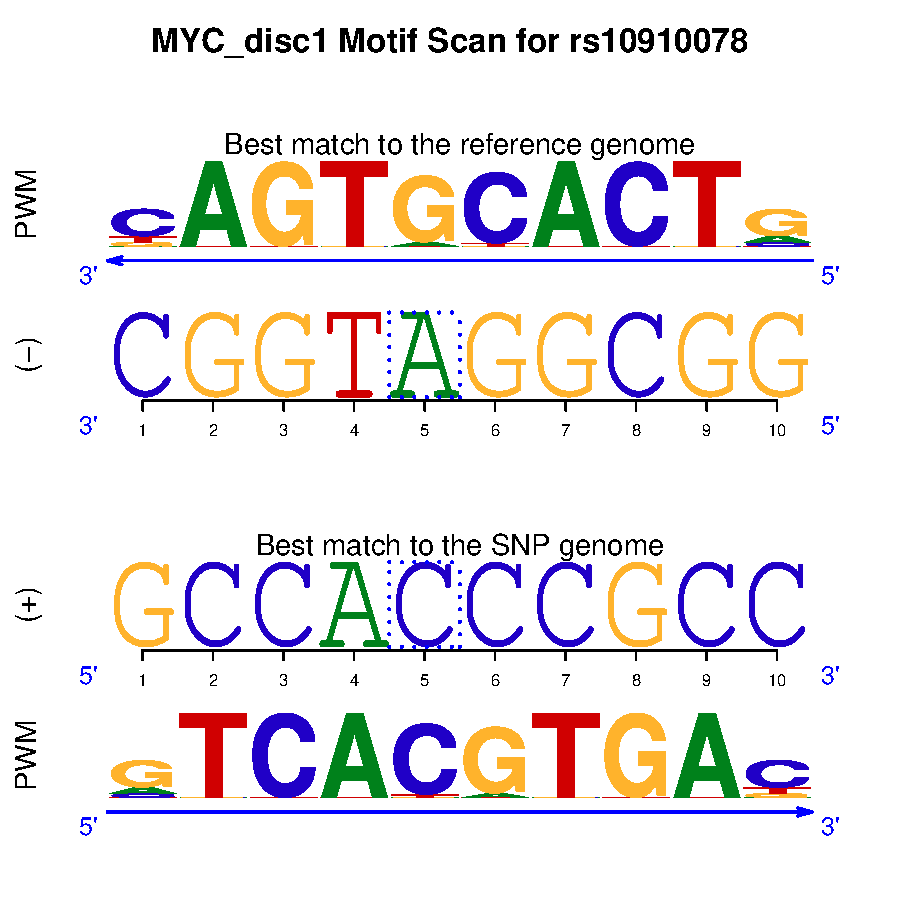
\includegraphics[width=\maxwidth]{figure/unnamed-chunk-27-1} 

}



\end{knitrout}

\section{Session Information}

\begin{knitrout}
\definecolor{shadecolor}{rgb}{0.969, 0.969, 0.969}\color{fgcolor}\begin{kframe}
\begin{verbatim}
## R version 3.1.1 (2014-07-10)
## Platform: x86_64-redhat-linux-gnu (64-bit)
## 
## locale:
##  [1] LC_CTYPE=zh_TW.UTF-8       LC_NUMERIC=C               LC_TIME=en_US.UTF-8       
##  [4] LC_COLLATE=en_US.UTF-8     LC_MONETARY=en_US.UTF-8    LC_MESSAGES=en_US.UTF-8   
##  [7] LC_PAPER=en_US.UTF-8       LC_NAME=C                  LC_ADDRESS=C              
## [10] LC_TELEPHONE=C             LC_MEASUREMENT=en_US.UTF-8 LC_IDENTIFICATION=C       
## 
## attached base packages:
## [1] grid      parallel  stats     graphics  grDevices utils     datasets  methods  
## [9] base     
## 
## other attached packages:
##  [1] SNPlocs.Hsapiens.dbSNP.20120608_0.99.9 atSNP_1.0                             
##  [3] motifStack_1.6.5                       ade4_1.6-2                            
##  [5] MotIV_1.18.0                           grImport_0.9-0                        
##  [7] XML_3.98-1.1                           doMC_1.3.3                            
##  [9] iterators_1.0.7                        foreach_1.4.2                         
## [11] data.table_1.9.4                       Rcpp_0.11.4                           
## [13] BSgenome.Hsapiens.UCSC.hg19_1.3.19     BSgenome_1.30.0                       
## [15] Biostrings_2.30.1                      GenomicRanges_1.14.4                  
## [17] XVector_0.2.0                          IRanges_1.20.7                        
## [19] BiocGenerics_0.8.0                     BiocInstaller_1.12.1                  
## 
## loaded via a namespace (and not attached):
##  [1] BiocStyle_1.0.0 chron_2.3-45    codetools_0.2-8 compiler_3.1.1  evaluate_0.5.5 
##  [6] formatR_1.0     highr_0.4       knitr_1.9       lattice_0.20-29 plyr_1.8.1     
## [11] reshape2_1.4.1  rGADEM_2.10.0   seqLogo_1.28.0  stats4_3.1.1    stringr_0.6.2  
## [16] tools_3.1.1
\end{verbatim}
\end{kframe}
\end{knitrout}


%\bibliographystyle{apalike}
%\bibliographystyle{natbib}

\bibliographystyle{plain}
\bibliography{document}

\end{document}
